\section{Content}
\label{section:content}

\subsection{DDoS Attacks and BRO}\label{subsec:ddos-and-bro}
In this section we will first define the notion of a DDoS attack by explaining how the infrastructure looks like. Then we will elaborate on various DDoS attacks used nowadays and discuss their main characteristics. After this we will discuss the syntax of the detection rules of the BRO SIDS.

\subsubsection{The DDoS Attack}
Figure \ref{fig:ddos-overview} shows the infrastructure of a DDoS attack. Actors involved in a DDoS attack are denoted by a letter (A-D) whereas data streams are denoted by numbers (1-5). 

A DDoS attack starts with an attacker (A). The attacker sends data needed to start the attack (1) to the Command and Control (C\&C) servers (B). The C\&C servers control the infected machines (C). The infected machines are also known under the name of bots. The C\&C servers plus the infected machines are more commonly named as a botnet. The C\&C servers send a message (2) to the infected machines. In case of the Ramnit botnet, only the infected machines counted 3.2 million machines \cite{europol2015}. At this point two paths are used to get to the target machine (E). The first path possible is aiming the infected machines directly to the target (4). The second path possible is using public services (D) like a DNS to reach the target (5). 

In the next subsection we will describe various types of DDoS attacks. 

\begin{figure}[H]
\centering
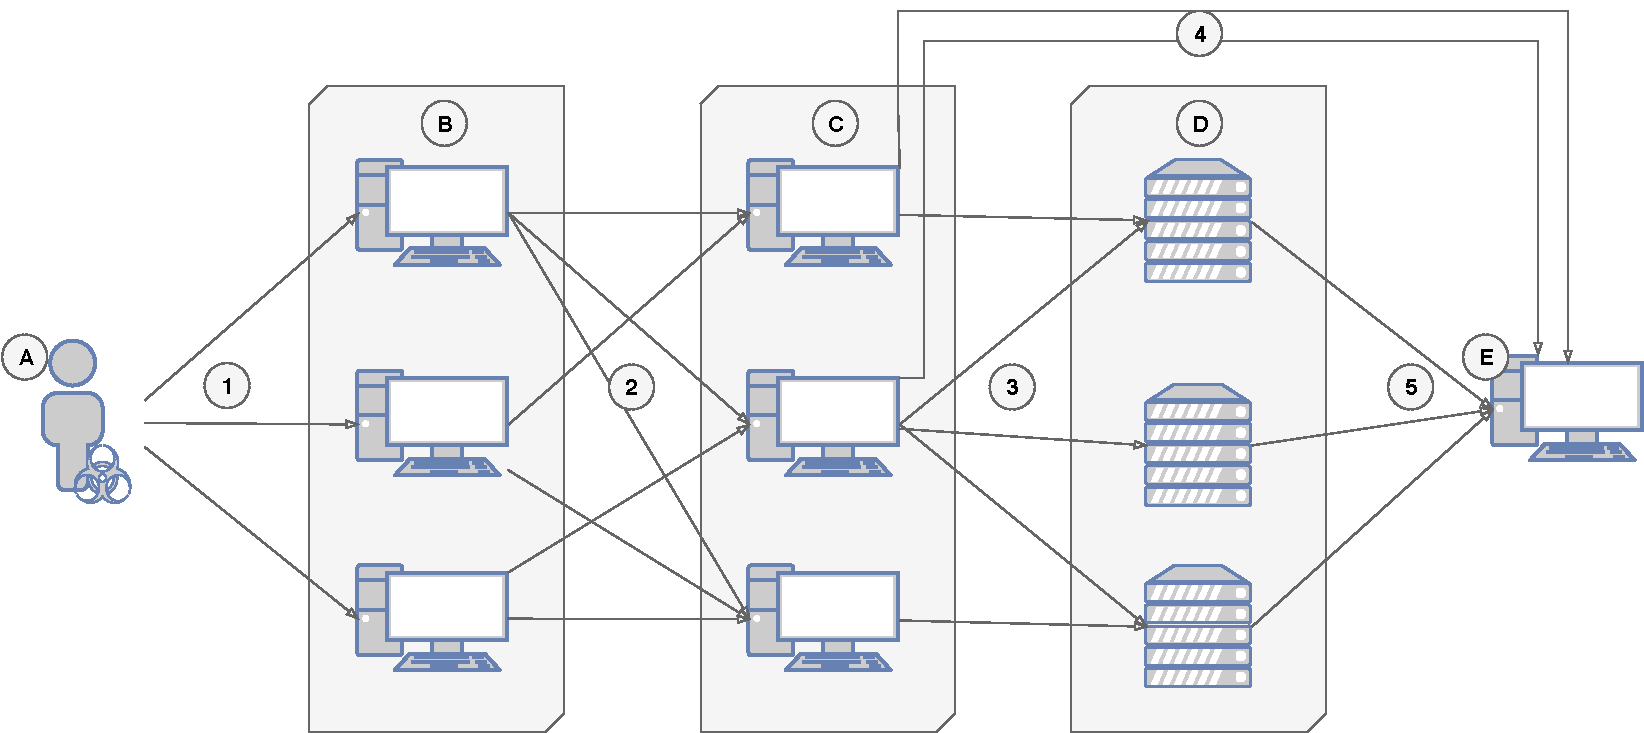
\includegraphics[width=\textwidth]{./images/ddos-overview.pdf}
\caption{Overview of DDoS attack infrastructure}
\end{figure}\label{fig:ddos-overview}

\subsubsection{Types of Attacks}
In this section we will briefly elaborate on various types of attack. The main characteristics can be found in Table $\dots$.

\paragraph{UDP Fragment}
The UDP Fragmantation attack exploits the fragmentation used in the IP protocol \cite{imperva}. When a packet is to big to be sent across a network link, it will be broken down into smaller packets and later on resembled again. In a UDP Fragmentation attack, fraudulent UDP packets are sent which are larger than the maximum transmission unit (MTU) of the network. The idea is that the packets can not be reassembled and thereby consuming the server's resources. 

\paragraph{DNS}
The DNS attack exploits the public DNS services on the internet. DNS is used to resolve IP adresses from website names. In a DNS attack the attacker spoofs its IP replacing its IP with that of the target. The DNS server sees the request as it came from the target and replies as if it were a normal request. This way of attacking allows an attacker to amplify its own bandwidth by using the asymmetry between request and response size. 

\paragraph{NTP}
The NTP attack exploits the public NTP services on the internet. NTP services allow for time synchronization between machines. This attack is similar to the DNS attack, but this time the NTP services are used. 

\paragraph{Chargen}
The Chargen attack exploits the public Character Generator Protocol (Chargen). Once a Chargen services receives a packet via UDP, it responds by sending a datagram containing a random number between 0 and 512 characters long \cite{ietf1983}. The attack approach works the same as the NTP and DNS attack.  






\subsubsection{BRO Rule Syntax} 


\subsection{Methodology}\label{subsec:methodology}

\subsection{Evaluation and Discussion}\label{subsec:evaluation-discussion}
\subsubsection{Evaluation}\label{subsubsec:evalutation}
\subsubsection{Discussion}\label{subsubsec:discussion}
